%! Author = ruochongli
%! Date = 2023/3/9

% Preamble
\documentclass[./main.tex]{subfiles}

% Packages

% Document
\begin{document}
    \section{Model Overview}
    In our model, we aim at three goals: making the profit as high as possible, lowering the financial risk caused by
    pollution, and protecting the environment as much as possible.

    To solve the problem, we firstly determined metrics which include both geological ones and human ones.
    Geological metrics are slope, vegetation coverage, humidity, precipitation, illumination, temperature and so on,
    while human metrics include revenue, maintenance cost, prime cost, employment, visitors flow rate and such.
    In our model, each metric is assigned with a weight $1$; however, the weight is highly changeable according to
    decision makers\rq\ demands.
    For facilities, we consider cross-country skiing facilities, crop farms, ranches, regenerative farms, and
    agritourist centers.

    Secondly, we get the suitability-time function.
    By using mathematical calculations, we can get the functions of these metrics changing throughout the time.
    Then, we multiply each function with certain conversion rate functions $h_c \left( t \right)$, and get different
    values representing how suitable it will be.

    After calculating every metrics in discrete time, we get discrete functions of time.
    Traverse the upper steps for every piece of land property, and we get different matrices from different aspects
    containing suitability-time function.

    Figure~\ref{fig:figureDiagram} is the algorithm of calculating the activity-time [$A\left(t\right)$] function and
    the metric-time [$\alpha\left(t\right)$] function.
    in the figure, $V$ is the impact of the metrics on the facility in its own position; $U$ is the impact of the
    facility on the value of the metrics; $W$ is weight of each metric to the facility.

    \begin{gather*}
        A\left( t \right)\xrightarrow[\alpha_{\left( t \right)}]{V, W}A\left( t+\mathrm{d}t \right)\\
        \alpha_{\left( t \right)}\xrightarrow[A\left( t \right)]{U_{\mathrm{type}_k, i}}\alpha_{\left( t+\mathrm{d}t
        \right)}\\
    \end{gather*}

    \begin{figure}[H]
        \centering
        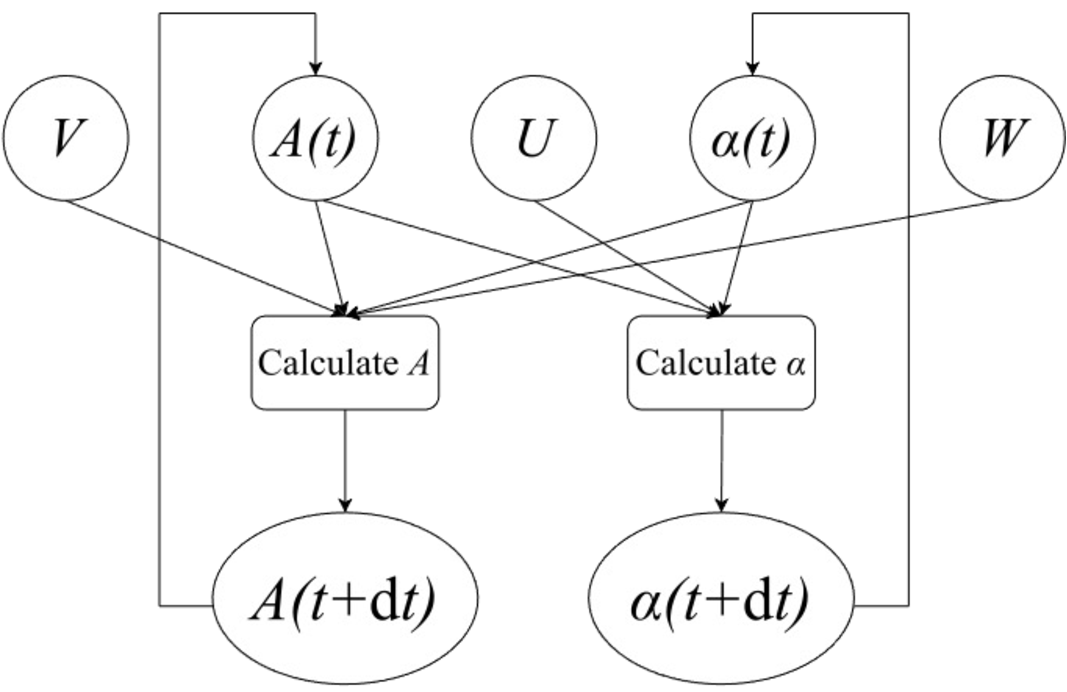
\includegraphics[width=0.5\textwidth]{./figure/figureDiagrams}
        \caption{The algorithm for calculating activity and metric function}
        \label{fig:figureDiagram}
    \end{figure}


    Overall, the algorithm can be summarized into the flowchart in Figure~\ref{fig:figureFlowchart}.
    In Figure~\ref{fig:figureFlowchart}, $A$ is the \lq\lq{activity}\rq\rq of the facilities, and $P$ is the coefficient
    of profit.

    \begin{figure}[H]
        \centering
        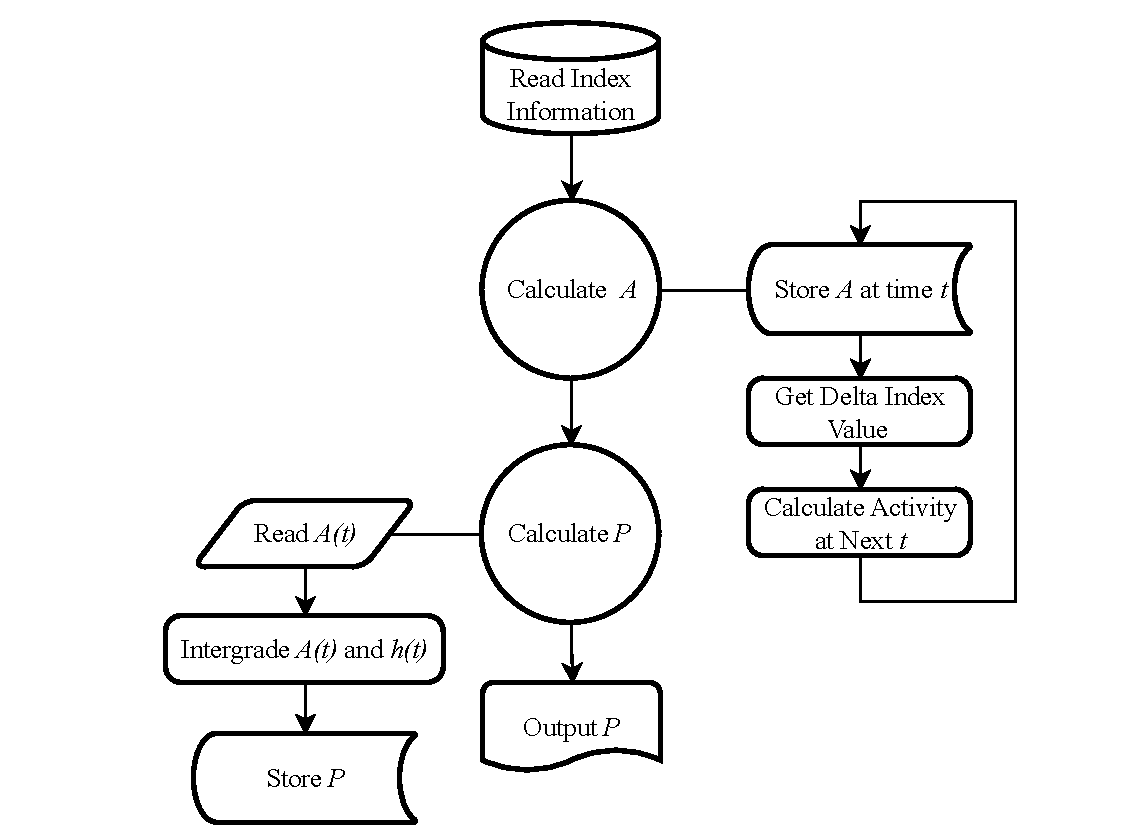
\includegraphics[width=0.75\textwidth]{./figure/figureFlowchart4}
        \caption{Flowchart of the algorithm}
        \label{fig:figureFlowchart}
    \end{figure}



\end{document}